%------------------------------------------------------------------------------------------------------------------------------------------------------------------------------------------
% The Beamer class comes with a number of default slide themes
% which change the colors and layouts of slides. Below this is a list
%------------------------------------------------------------------------------------------------------------------------------------------------------------------------------------------
% of all the themes, uncomment each in turn to see what they look like.% As well as themes, the Beamer class has a number of color themes
% for any slide theme. Uncomment each of these in turn to see how it
% changes the colors of your current slide theme.
%------------------------------------------------------------------------------------------------------------------------------------------------------------------------------------------
%----------------------------------------------------------------------------------------
%	Packages
%----------------------------------------------------------------------------------------
\documentclass{beamer}
\usepackage{graphicx}
\usepackage{booktabs} % Allows the use of \toprule, \midrule and \bottomrule in tables
\usepackage{multicol}
\usepackage{braket}
\graphicspath{{Figures/}}
\mode<presentation> {
%----------------------------------------------------------------------------------------
%	Templates
%----------------------------------------------------------------------------------------
%\setbeamertemplate{footline} % To remove the footer line in all slides uncomment this line
\setbeamertemplate{footline}[page number] % To replace the footer line in all slides with a simple slide count uncomment this line
\setbeamertemplate{navigation symbols}{} % To remove the navigation symbols from the bottom of all slides uncomment this line
%----------------------------------------------------------------------------------------
%	Themes
%----------------------------------------------------------------------------------------
%\usetheme{default}
%\usetheme{AnnArbor}
%\usetheme{Antibes}
%\usetheme{Bergen}
%\usetheme{Berkeley}
%\usetheme{Berlin}
%\usetheme{Boadilla}
%\usetheme{CambridgeUS}
%\usetheme{Copenhagen}
%\usetheme{Darmstadt}
%\usetheme{Dresden}
%\usetheme{Frankfurt}
%\usetheme{Goettingen}
%\usetheme{Hannover}
%\usetheme{Ilmenau}
%\usetheme{JuanLesPins}
%\usetheme{Luebeck}
%\usetheme{Madrid}
%\usetheme{Malmoe}
\usetheme{Marburg}
%\usetheme{Montpellier}
%\usetheme{PaloAlto}
%\usetheme{Pittsburgh}
%\usetheme{Rochester}
%\usetheme{Singapore}
%\usetheme{Szeged}
%\usetheme{Warsaw}
%----------------------------------------------------------------------------------------
%	Color Themes
%----------------------------------------------------------------------------------------
%\usecolortheme{albatross}
%\usecolortheme{beaver}
%\usecolortheme{beetle}
%\usecolortheme{crane}
%\usecolortheme{dolphin}
%\usecolortheme{dove}
%\usecolortheme{fly}
\usecolortheme{lily}
%\usecolortheme{orchid}
%\usecolortheme{rose}
%\usecolortheme{seagull}
%\usecolortheme{seahorse}
%\usecolortheme{whale}
%\usecolortheme{wolverine}
}
%----------------------------------------------------------------------------------------
%	TITLE PAGE
%----------------------------------------------------------------------------------------
\title{Improving Quantum Parameter Estimation} % The short title appears at the bottom of every slide, the full title is only on the title page
\author{Taylor Larrechea} % Your name
\institute[CMU] % Your institution as it will appear on the bottom of every slide, may be shorthand to save space
{
Colorado Mesa University \\ % Your institution for the title page
\medskip
}
\date{April 30, 2020} % Date, can be changed to a custom date
%----------------------------------------------------------------------------------------
%	Begin Document
%----------------------------------------------------------------------------------------
\begin{document}
\begin{frame}
\titlepage % Print the title page as the first slide
\end{frame}
%----------------------------------------------------------------------------------------
%	Presentation Slides
%----------------------------------------------------------------------------------------
%------------------------------------------------
%	Table of Contents
%------------------------------------------------
\begin{frame}
\frametitle{Table of Contents}
\begin{multicols}{2}
\tableofcontents
\end{multicols}
\end{frame}
%----------------------------------------------------------------------------------------------------------------------------------------------------
%------------------------------------------------
%	What is Quantum Estimation (Spin-1/2 Particles)
%------------------------------------------------
\section{What is Quantum Estimation?}
\begin{frame}
\frametitle{Spin-1/2 Particles}
Quantum estimation is the use of quantum mechanical systems as measuring devices for physical parameters.
\begin{figure}
\begin{center}
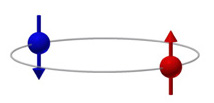
\includegraphics[width=0.75\linewidth]{Spin-12-Cartoon.jpg}
\end{center}
\end{figure}
In the context of this presentation, these quantum mechanical systems are spin-1/2 particles.
\end{frame}
%------------------------------------------------
%	What is Quantum Estimation (Spin-1/2 Particles in Magnetic Field)
%------------------------------------------------
\subsection{\tiny{Spin-1/2 Particles}}
\begin{frame}
\frametitle{Spin-1/2 Particles in Magnetic Field}
These spin-1/2 particles can be subjected to something like a magnetic field. 
\begin{figure}
\begin{center}
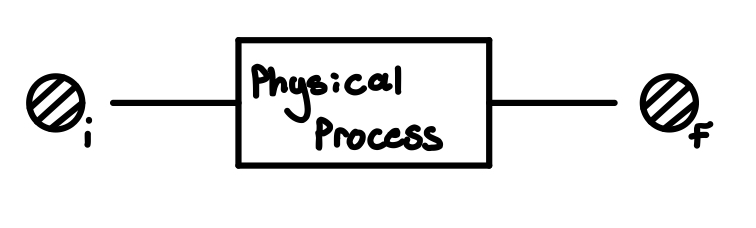
\includegraphics[width=0.75\linewidth]{Spin-12-In-Magnetic-Field.jpeg}
\end{center}
\end{figure}
Can measure the change in the spin vector.
\end{frame}
%------------------------------------------------
%	What is Quantum Estimation (Example of Quantum Estimation)
%------------------------------------------------
\begin{frame}
\frametitle{Example of Quantum Estimation}
An example of spin-1/2 particles and parameters is in MRI machines.
\begin{figure}
\begin{center}
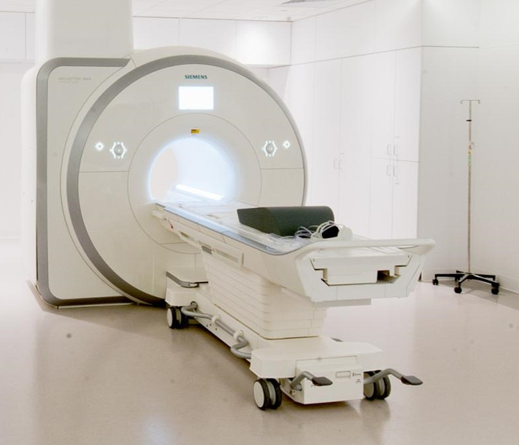
\includegraphics[width=0.75\linewidth]{MRI-Machine.png}
\end{center}
\end{figure}
\end{frame}
%----------------------------------------------------------------------------------------------------------------------------------------------------
%------------------------------------------------
%	What is Estimation (Estimation)
%------------------------------------------------
\section{What is Estimation?}
\begin{frame}
\frametitle{Estimation}
\begin{figure}
\begin{center}
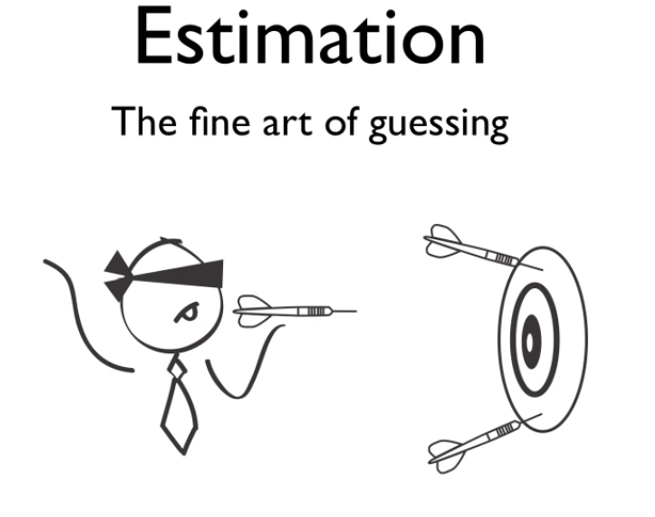
\includegraphics[width=0.75\linewidth]{Estimation-Cartoon.png}
\end{center}
\end{figure}
\end{frame}
%------------------------------------------------
%	What is Estimation (Coin Toss)
%------------------------------------------------
\subsection{\tiny{Coin Toss}}
\begin{frame}
\frametitle{Coin Toss}
The simplest example of estimation is a coin toss.
\begin{figure}
\begin{center}

\includegraphics[width=0.75\linewidth]{Coin-Flip-Cartoon.jpeg}
\end{center}
\end{figure}
The result of this coin flip is either heads or tails.
\end{frame}
%------------------------------------------------
%	What is Estimation (Probability)
%------------------------------------------------
\begin{frame}
\frametitle{Probability}
Wish to estimate the probability of obtaining heads. \\
\vspace{10pt}
$N$ is the number of times flipped,  $n_H$ is how many times heads appears. \\
\vspace{10pt}
Probability estimate of obtaining heads is
\begin{equation}\label{eq:1}
P_{est}=\frac{n_H}{N}.
\end{equation}
\end{frame}
%------------------------------------------------
%	What is Estimation (Fluctuating Estimates)
%------------------------------------------------
\begin{frame}
\frametitle{Fluctuating Estimates}
Multiple runs of $\textit{N}$ flips will give different estimates. \\
\vspace{10pt}
Fluctuation of estimates is calculated via
\begin{equation}\label{eq:2}
\nu=\bar{P}^2_{est}-(\bar{P}_{est})^2.
\end{equation}
$\bar{P^2}_{est}$ and $\bar{P}_{est}$ are calculated via
\begin{equation}\label{eq:3}
\bar{P}_{est}=\frac{1}{N}\bar{n}_H \hspace{25pt} \text{and} \hspace{25pt} \bar{P}^2_{est}=\frac{1}{N^2}\bar{n}^2_{H}.
\end{equation}
We aim to have the smallest variance possible.
\end{frame}
%------------------------------------------------
%	What is Estimation (Variance and Fisher Information)
%------------------------------------------------
\begin{frame}
\frametitle{Variance and Fisher Information}
The variance binomial outcomes is 
\begin{equation}\label{eq:4}
\nu=\frac{P_{est}}{N}(1-P_{est}).
\end{equation}
The Fisher Information is calculated via
\begin{equation}\label{eq:5}
F=\sum_{\text{\tiny{All Possible Outcomes}}}^{\infty}\frac{1}{\text{\tiny{Prob(Outcome)}}}\bigg(\frac{\partial \text{\tiny{Prob(Outcome)}}}{\partial \text{P}}\bigg)^2.
\end{equation}
The Cramer-Rao bound tells us that
\begin{equation}\label{eq:6}
\nu\geq\frac{1}{F}.
\end{equation}
where $F$ is calculated in equation (\ref{eq:5}). The Fisher Information of our coin flip experiment via
\begin{equation}\label{eq:7}
F_{\text{\tiny{N Toss}}}=N\cdot F_{\text{\tiny{Single Toss}}}=N\cdot\frac{1}{P(1-P)}=\frac{N}{P(1-P)}.
\end{equation}
\end{frame}
%----------------------------------------------------------------------------------------------------------------------------------------------------
%------------------------------------------------
%	Quantum Systems (Single Particles)
%------------------------------------------------
\section{Quantum Systems}
\subsection{\tiny{Single Particle}}
\begin{frame}
\frametitle{Single Particles}
The state of a single particle mathematically is represented by
\begin{equation}\label{eq:8}
\ket{+\hat{n}}=\cos{(\theta/2)}\ket{0}+e^{i\phi}\sin{(\theta/2)}\ket{1}
\end{equation}
and
\begin{equation} \label{eq:9}
\ket{-\hat{n}}=\sin{(\theta/2)}\ket{0}-e^{i\phi}\cos{(\theta/2)}\ket{1}.
\end{equation}
\begin{figure}
\begin{center}
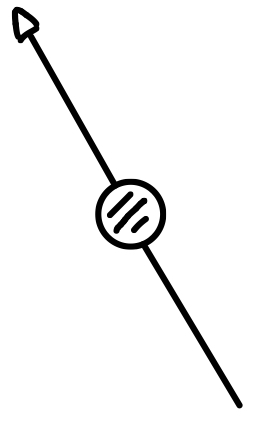
\includegraphics[width=0.20\linewidth]{Single-Particle.jpeg}
\end{center}
\end{figure}
\end{frame}
%------------------------------------------------
%	Quantum Systems (Unitary Evolution)
%------------------------------------------------
\subsection{\tiny{Unitary Evolution}}
\begin{frame}
\frametitle{Unitary Evolution}
States can evolve via physical processes, mathematically this is calculated by
\begin{equation}\label{eq:10}
\ket{\psi_f}=\hat{U}\ket{\psi_i}.
\end{equation}
\begin{figure}
\begin{center}
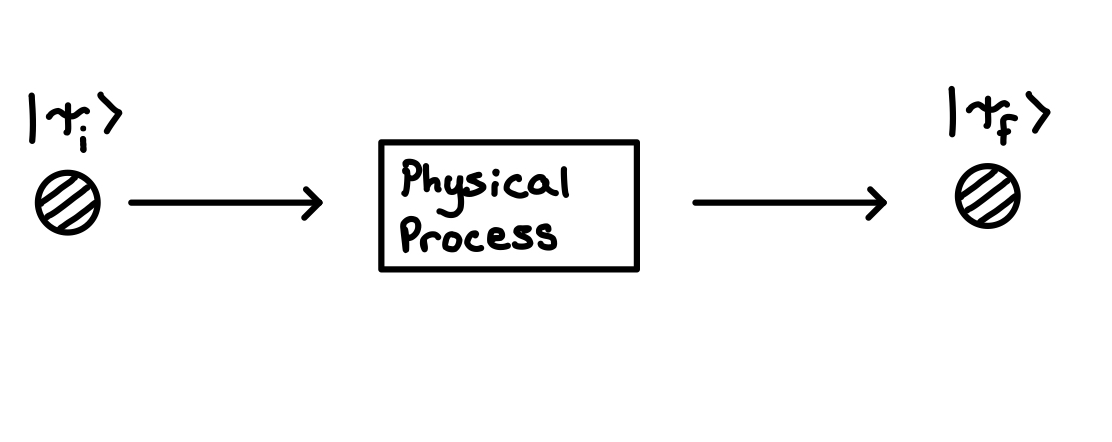
\includegraphics[width=0.75\linewidth]{Unitary-Operator.PNG}
\end{center}
\end{figure}
It should be noted that $\hat{U}$ are $2^n\times2^n$ matrices where $n$ is the number of particles.
\end{frame}
%------------------------------------------------
%	Quantum Systems (Unitary Parameter Evolution)
%------------------------------------------------
\begin{frame}
\frametitle{Unitary Parameter Evolution}
This evolution is calculated by
\begin{equation}\label{eq:11}
\ket{\psi_f}=\hat{U}(\lambda)\ket{\psi_i}.
\end{equation}
An example of this unitary operator is
\begin{equation}\label{eq:12}
\hat{U}(\lambda)=
\begin{pmatrix}
e^{-i\lambda/2} & 0 \\
0 & e^{i\lambda/2}
\end{pmatrix}.
\end{equation}
\begin{equation}\label{eq:13}
\ket{\psi_i}=\frac{1}{\sqrt{2}}(\ket{0}+\ket{1}) \rightarrow \ket{\psi_f}=\frac{1}{\sqrt{2}}(e^{-i\lambda/2}\ket{0}+e^{i\lambda/2}\ket{1})
\end{equation}
$\lambda$ is the parameter that we wish to estimate.
\end{frame}
%------------------------------------------------
%	Quantum Systems (Multiple Particles)
%------------------------------------------------
\subsection{\tiny{Multiple Particles}}
\begin{frame}
\frametitle{Multiple Particles}
We can now discuss quantum systems with multiple particles.
\begin{figure}
\begin{center}
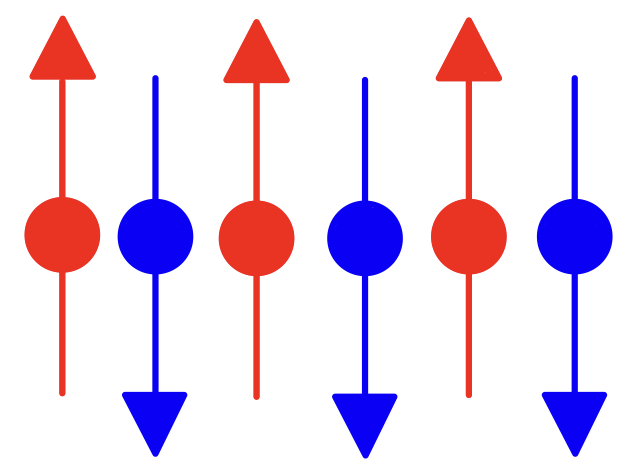
\includegraphics[width=0.75\linewidth]{Spin-12-System.jpg}
\end{center}
\end{figure}
\end{frame}
%------------------------------------------------
%	Quantum Systems (Product States)
%------------------------------------------------
\begin{frame}
\frametitle{Product States}
A generic state is
\begin{equation}\label{eq:14}
\ket{\psi}=c_0\ket{0}\ket{0}+c_1\ket{0}\ket{1}+c_2\ket{1}\ket{0}+c_3\ket{1}\ket{1}.
\end{equation}
A product state can be written as
\begin{equation}\label{eq:15}
\ket{\psi}=\ket{\psi_A}\ket{\psi_B}.
\end{equation}
An example is
\begin{equation}\label{eq:16}
\ket{\psi}=\frac{1}{\sqrt{2}}(\ket{0}-\ket{1})\cdot\frac{1}{\sqrt{2}}(\ket{0}+\ket{1})
\end{equation}
where
\begin{equation}\label{eq:17}
\ket{\psi}=\frac{1}{2}(\ket{0}\ket{0}+\ket{0}\ket{1}-\ket{1}\ket{0}-\ket{1}\ket{1}).
\end{equation}
\end{frame}
%------------------------------------------------
%	Quantum Systems (Entangled States)
%------------------------------------------------
\begin{frame}
\frametitle{Entangled States}
An example of an entangled state is
\begin{equation}\label{eq:18}
\ket{\psi}=\frac{1}{2}(\ket{0}\ket{0}+\ket{0}\ket{1}+\ket{1}\ket{0}-\ket{1}\ket{1})
\end{equation}
Entangled states do not exist in classical physics.
\begin{figure}
\begin{center}
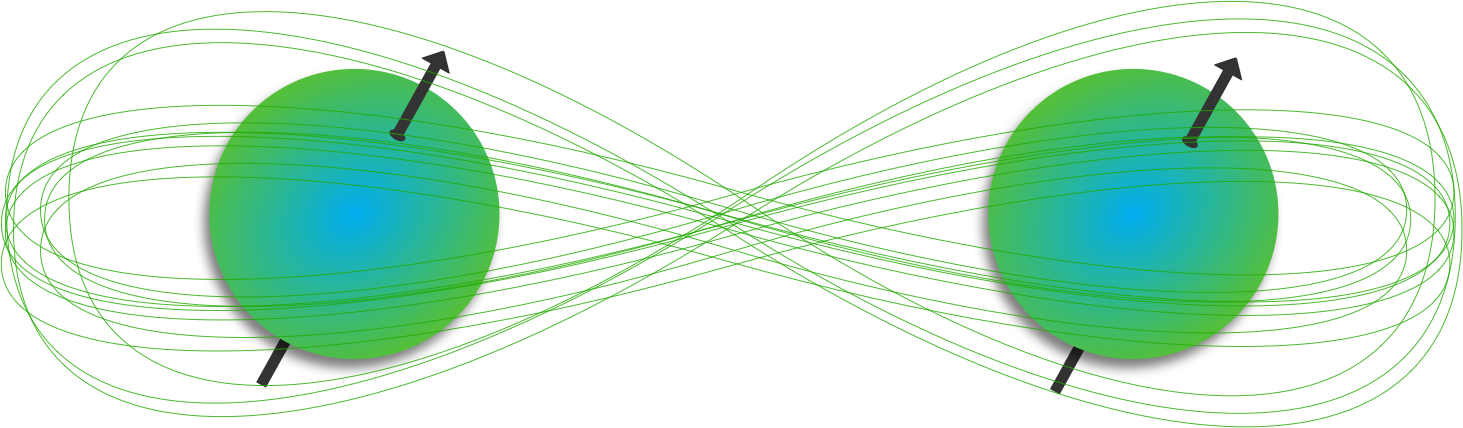
\includegraphics[width=0.75\linewidth]{Entangled-States-Description.png}
\end{center}
\end{figure}
\end{frame}
%------------------------------------------------
%	Quantum Systems (Density Operators)
%------------------------------------------------
\subsection{\tiny{Density Operators}}
\begin{frame}
\frametitle{Density Operators}
Exact state unknown. Represented by state $\ket{\psi_1}$ with probability $a_1$ and $\ket{\psi_2}$ with probability $a_2$
\begin{equation}\label{eq:19}
\hat{\rho}=a_1\ket{\psi_1}\bra{\psi_1}+a_2\ket{\psi_2}\bra{\psi_2}.
\end{equation}
For example
\begin{equation}\label{eq:20}
\ket{\psi_1}=\frac{1}{\sqrt{2}}(\ket{0}+\ket{1}) \hspace{2pt} \text{with} \hspace{2pt} a_1=\frac{1+r}{2}
\end{equation}
\begin{equation}\label{eq:21}
\ket{\psi_2}=\frac{1}{\sqrt{2}}(\ket{0}-\ket{1}) \hspace{2pt} \text{with} \hspace{2pt} a_2=\frac{1-r}{2}
\end{equation}
the density operator is then
\begin{equation}\label{eq:22}
\hat{\rho}=\frac{1}{2}
\begin{pmatrix}
1 & r \\
r & 1
\end{pmatrix}.
\end{equation}
Equation (\ref{eq:22}) is the density operator that will be used without the rest of the talk.
\end{frame}
%------------------------------------------------
%	Quantum Systems (Density Operators With Parameters)
%------------------------------------------------
\begin{frame}
\frametitle{Density Operators With Parameters}
Parameter dependent density operators evolve via
\begin{equation}\label{eq:23}
\hat{\rho}(\lambda)=\hat{U}(\lambda)\hat{\rho}_0\hat{U}^{\dagger}(\lambda)
\end{equation}
An example 
\begin{equation}\label{eq:24}
\hat{U}(\lambda)=
\begin{pmatrix}
e^{-i\lambda/2} & 0 \\
0 & e^{i\lambda/2} \\
\end{pmatrix}
\hspace{10pt} \text{and} \hspace{10pt}
\hat{\rho}_0=\frac{1}{2}
\begin{pmatrix}
1 & r \\
r & 1
\end{pmatrix}
\end{equation}
then evolves to
\begin{equation}\label{eq:25}
\hat{\rho}_f=\frac{1}{2}
\begin{pmatrix}
1 & re^{-i\lambda} \\
re^{i\lambda} & 1
\end{pmatrix}.
\end{equation}
\end{frame}
%----------------------------------------------------------------------------------------------------------------------------------------------------
%------------------------------------------------
%	Quantum Estimation
%------------------------------------------------
\section{Quantum Estimation}
\subsection{\tiny{QFI Definition}}
\begin{frame}
\frametitle{Quantum Estimation}
A key component of quantum estimation is called the Quantum Fisher Information.
\begin{figure}
\begin{center}
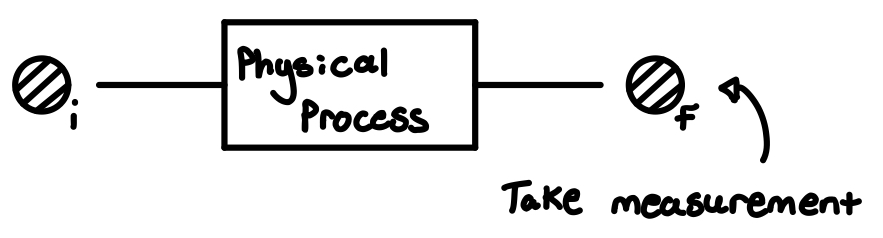
\includegraphics[width=0.75\linewidth]{Quantum-Estimation-Cartoon.jpeg}
\end{center}
\end{figure}
Relationship between $F$ and $H$ is
\begin{equation}\label{eq:26}
F\leq H.
\end{equation}
$H$ is not dependent upon measurement choice, only initial state.
\end{frame}
%------------------------------------------------
%	Quantum Estimation (QFI Calculation)
%------------------------------------------------
\subsection{\tiny{QFI Calculation}}
\begin{frame}
\frametitle{QFI Calculation}
The way this Quantum Fisher Information is calculated is by
\begin{equation}\label{eq:24}
H=\text{Tr}[\hat{\rho}\hat{L}^2]
\end{equation}
where 
\begin{equation}\label{eq:25}
\frac{\partial\hat{\rho}}{\partial\lambda}=\frac{1}{2}\big[\hat{\rho}\hat{L}+\hat{L}\hat{\rho}\big].
\end{equation}
Want to maximize Quantum Fisher Information.
\end{frame}
%------------------------------------------------
%	Quantum Estimation (Phase Shifts)
%------------------------------------------------
\subsection{\tiny{Phase Shifts}}
\begin{frame}
\frametitle{Phase Shifts}
We wish to estimate parameter $\lambda$ with $\hat{\rho}_f=\hat{U}(\lambda)\hat{\rho}_i\hat{U}(\lambda)^{\dagger}$.
\begin{equation}\label{eq:29}
\hat{\rho}_i=\frac{1}{2}
\begin{pmatrix}
1+r_{zi} & r_{xi}-ir_{yi} \\
r_{xi}+ir_{yi} & 1-r_{zi} \\
\end{pmatrix}
\end{equation}
Where $\hat{\rho}_f$ is
\begin{equation}\label{eq:30}
\hat{\rho}_f = \frac{1}{2}
\begin{pmatrix}
1+r_{zf} & r_{xf}-r_{yf} \\
r_{xf}+r_{yf} & 1-r_{zf}  \\
\end{pmatrix}
\end{equation}
Where
\begin{align}\label{eq:31}
r_{xf}&=r_{xi}\cos({\lambda})-r_{yi}\sin({\lambda}) \nonumber \\
r_{yf}&=r_{xi}\sin({\lambda})+r_{yi}\cos({\lambda}) \\
r_{zf}&=r_{zi}. \nonumber 
\end{align}
\end{frame}
%------------------------------------------------
%	Quantum Estimation (Visualizing of Phase Shifts)
%------------------------------------------------
\begin{frame}
\frametitle{Visualizing of Phase Shifts}
We can picture this Phase Shift in the figure.
\begin{figure}
\begin{center}
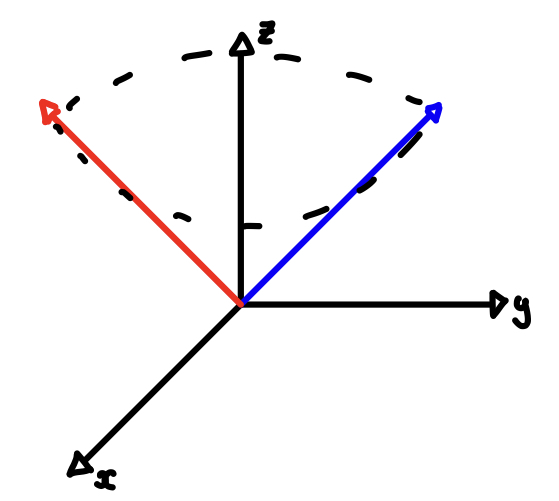
\includegraphics[width=0.75\linewidth]{Phase-Shift-Modeling.jpeg}
\end{center}
\end{figure}
\end{frame}
%------------------------------------------------
%	Quantum Estimation (One Particle Phase Shift)
%------------------------------------------------
\begin{frame}
\frametitle{One Particle Phase Shift}
We now examine single particle phase shifts.
\begin{figure}
\begin{center}
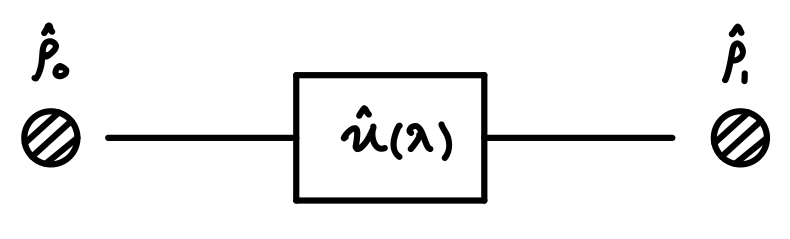
\includegraphics[width=0.75\linewidth]{One-Particle-QFI.jpg}
\end{center}
\end{figure}
The Quantum Fisher Information is
\begin{equation}\label{eq:32}
H=r^2.
\end{equation}
\end{frame}
%------------------------------------------------
%	Quantum Estimation (Two Particle one Channel Phase Shift)
%------------------------------------------------
\begin{frame}
\frametitle{Two Particle one Channel Phase Shift}
We now examine a two particle phase shift.
\begin{figure}
\begin{center}
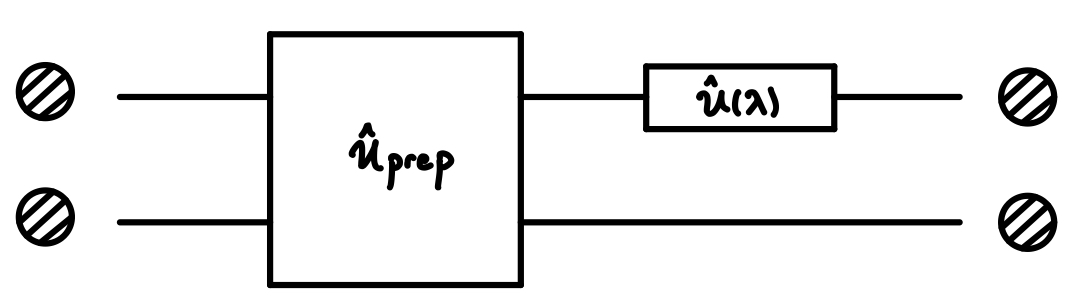
\includegraphics[width=0.75\linewidth]{Two-Particle-QFI.jpg}
\end{center}
\end{figure}
The $\hat{U}_{prep}$ matrix involves single qubit operations, one interaction is between two particles. \\ 
\vspace{10pt}
The Quantum Fisher Information is
\begin{equation}\label{eq:33}
H=\frac{2r^2}{1+r^2}.
\end{equation}
\end{frame}
%------------------------------------------------
%	Quantum Estimation (Gain of Phase Shifts)
%------------------------------------------------
\begin{frame}
\frametitle{Gain of Phase Shifts}
One can calculate what is called the gain of two scenarios by $G=\frac{H_{both}}{H_{single}}$. The gain of the last two scenarios is 
\begin{equation}\label{eq:34}
G=\frac{2}{1+r^2}.
\end{equation}
\begin{figure}
\begin{center}
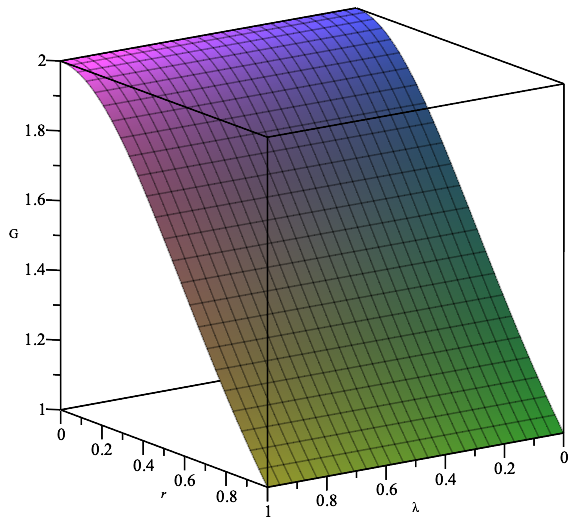
\includegraphics[width=0.55\linewidth]{Simple-Scenario-Gain.png}
\end{center}
\end{figure}
When $G>1$ the correlated scheme is estimating better.
\end{frame}
%------------------------------------------------
%	Quantum Estimation (Phase Flips)
%------------------------------------------------
\subsection{\tiny{Phase Flips}}
\begin{frame}
\frametitle{Phase Flips}
We wish to estimate parameter $\lambda$ with $\hat{\rho}_f=(1-\lambda)\hat{\rho}_i+\lambda\hat{\sigma}_z\hat{\rho}_i\hat{\sigma}_z$.
\begin{equation}\label{eq:35}
\hat{\rho}_i=\frac{1}{2}
\begin{pmatrix}
1+r_{zi} & r_{xi}-ir_{yi} \\
r_{xi}+ir_{yi} & 1-r_{zi} \\
\end{pmatrix}
\end{equation}
Where $\hat{\rho}_f$ is
\begin{equation}\label{eq:36}
\hat{\rho}_f=\frac{1}{2}
\begin{pmatrix}
1+r_{zi} & (1-2\lambda)(r_{xi}-ir_{yi}) \\
(1-2\lambda)(r_{xi}+ir_{yi}) & 1-r_{zi} \\
\end{pmatrix}.
\end{equation}
The evolution of each component of these particles is
\begin{align}\label{eq:37}
r_{xf}&=r_{xi}(1-2\lambda) \nonumber \\
r_{yf}&=r_{yi}(1-2\lambda) \\
r_{zf}&=r_{zi}. \nonumber
\end{align}
\end{frame}
%------------------------------------------------
%	Quantum Estimation (Visualizing of Phase Flips)
%------------------------------------------------
\begin{frame}
\frametitle{Visualizing of Phase Flips}
We can visualize how this Phase Flip evolves in the figure.
\begin{figure}
\begin{center}
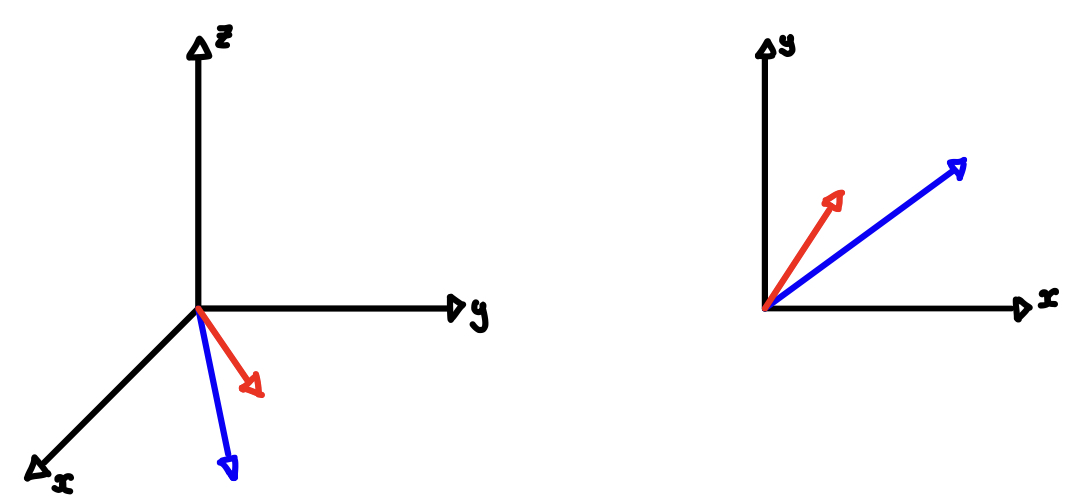
\includegraphics[width=0.90\linewidth]{Modeling-Of-Phase-Flip.jpeg}
\end{center}
\end{figure}
\end{frame}
%------------------------------------------------
%	Quantum Estimation (QFI of Phase Flips)
%------------------------------------------------
\begin{frame}
\frametitle{QFI of Phase Flips}
We examine the simplest scenario for a phase flip.
\begin{figure}
\begin{center}
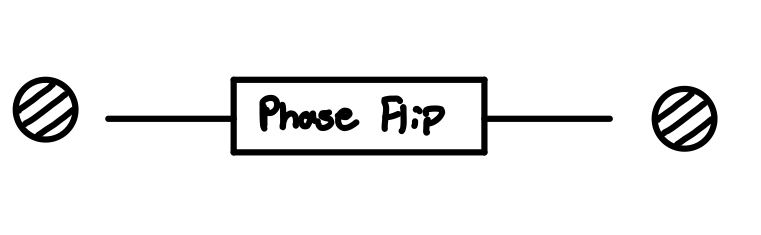
\includegraphics[width=0.60\linewidth]{Single-Particle-Phase-Flip-Evolution-Schematic.jpg}
\end{center}
\end{figure}
The Quantum Fisher Information is
\begin{equation}\label{eq:38}
H=\frac{4r^2}{1-r^2(1-2\lambda)^2}.
\end{equation}
\end{frame}
%------------------------------------------------
%	Quantum Estimation (QFI of Phase Flips Cont.)
%------------------------------------------------
\begin{frame}
\frametitle{QFI of Phase Flips Cont.}
The next scenario is with two particles, one channel phase flip.
\begin{figure}
\begin{center}
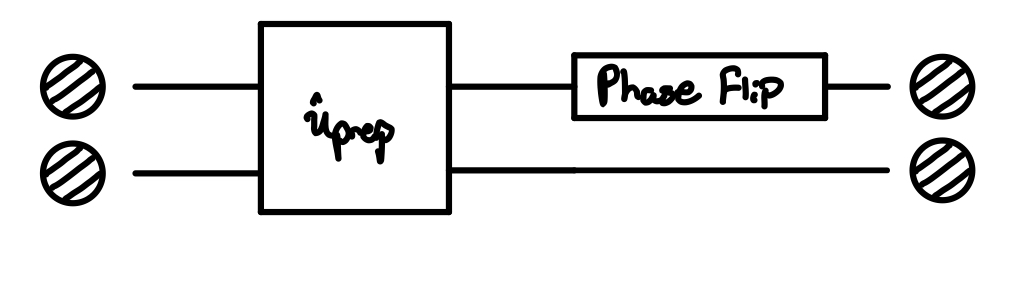
\includegraphics[width=0.60\linewidth]{Two-Particle-Phase-Flip-Single-Channel-Lambda-Schematic.jpeg}
\end{center}
\end{figure}
The Quantum Fisher Information is
\begin{equation}\label{eq:39}
H=\frac{8r^2(1+r^2)}{(1+r^2)^2-4r^2(1-2\lambda)^2}.
\end{equation}
\end{frame}
%------------------------------------------------
%	Quantum Estimation (QFI of Phase Flips Cont.)
%------------------------------------------------
\begin{frame}
\frametitle{QFI of Phase Flips Cont.}
The gain of the last two scenarios is
\begin{equation}\label{eq:40}
G=\frac{2(1+r^2)(1-r^2(1-2\lambda)^2)}{(1+r^2)^2-4r^2(1-2\lambda)^2}.
\end{equation}
\begin{figure}
\begin{center}
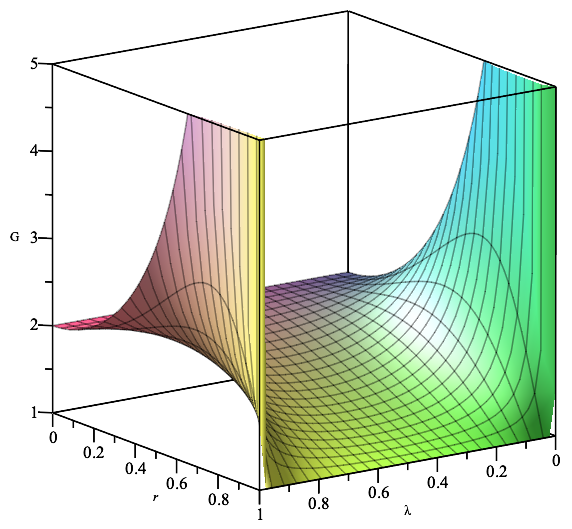
\includegraphics[width=0.50\linewidth]{Phase-Flip-One-Channel-Lambda-and-r-Gain.png}
\end{center}
\end{figure}
\end{frame}
%------------------------------------------------
%	Quantum Estimation (QFI of Phase Flips Cont.)
%------------------------------------------------
\begin{frame}
\frametitle{QFI of Phase Flips Cont.}
We now examine calculating the Quantum Fisher Information of a measurement with noise in a spectator.
\begin{figure}
\begin{center}
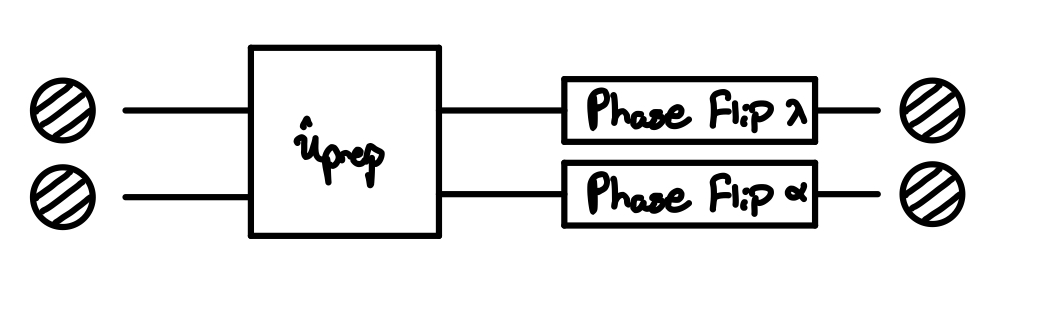
\includegraphics[width=0.75\linewidth]{Two-Particle-Phase-Flip-Dual-Channel-Alpha-Lambda-Schematic.jpg}
\end{center}
\end{figure}
The Quantum Fisher Information is
\begin{equation}\label{eq:41}
H=\frac{8r^2(1-2\alpha)^2(1+r^2)}{(1+r^2)^2-4r^2(1-2\lambda)^2(1-2\alpha)^2}.
\end{equation}
\end{frame}
%------------------------------------------------
%	Quantum Estimation (QFI of Phase Flips Cont.)
%------------------------------------------------
\begin{frame}
\frametitle{QFI of Phase Flips Cont.}
The gain of the last scenario is
\begin{equation}\label{eq:42}
G=\frac{2(1-2\alpha)^2(1+r^2)(1-r^2(1-2\lambda)^2)}{(1+r^2)^2-4r^2(1-2\lambda)^2(1-2\alpha)^2}.
\end{equation}
We will examine gains of when $\alpha=0.01, 0.1, 0.3, 0.5$.
\end{frame}
%------------------------------------------------
%	Quantum Estimation (QFI of Phase Flips Cont.)
%------------------------------------------------
\begin{frame}
\frametitle{QFI of Phase Flips Cont.}
Gain of when $\alpha=0.01$.
\begin{figure}
\begin{center}
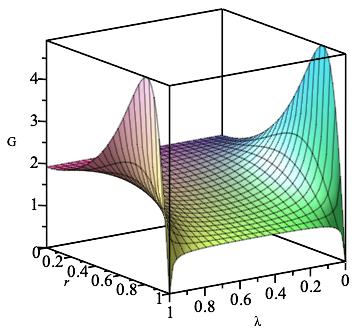
\includegraphics[width=0.75\linewidth]{Phase-Flip-Two-Channel-Alpha=001-Gain.png}
\end{center}
\end{figure}
\end{frame}
%------------------------------------------------
%	Quantum Estimation (QFI of Phase Flips Cont.)
%------------------------------------------------
\begin{frame}
\frametitle{QFI of Phase Flips Cont.}
Gain of when $\alpha=0.1$.
\begin{figure}
\begin{center}
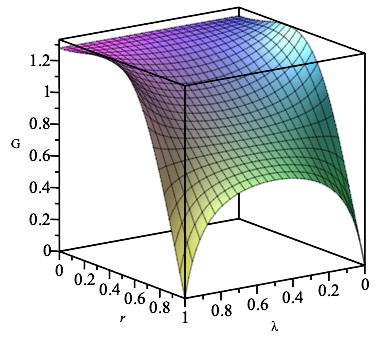
\includegraphics[width=0.75\linewidth]{Phase-Flip-Two-Channel-Alpha=01-Gain.png}
\end{center}
\end{figure}
\end{frame}
%------------------------------------------------
%	Quantum Estimation (QFI of Phase Flips Cont.)
%------------------------------------------------
\begin{frame}
\frametitle{QFI of Phase Flips Cont.}
Gain of when $\alpha=0.3$.
\begin{figure}
\begin{center}
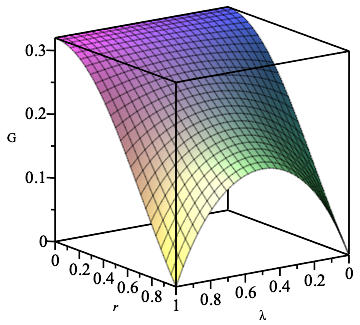
\includegraphics[width=0.75\linewidth]{Phase-Flip-Two-Channel-Alpha=03-Gain.png}
\end{center}
\end{figure}
\end{frame}
%------------------------------------------------
%	Quantum Estimation (QFI of Phase Flips Cont.)
%------------------------------------------------
\begin{frame}
\frametitle{QFI of Phase Flips Cont.}
Gain of when $\alpha=0.5$.
\begin{figure}
\begin{center}
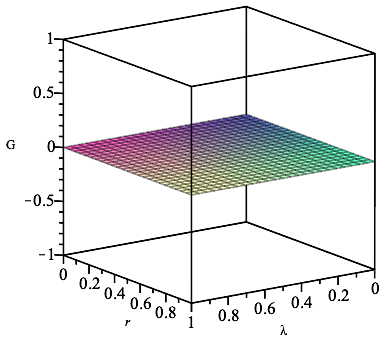
\includegraphics[width=0.75\linewidth]{Phase-Flip-Two-Channel-Alpha=05-Gain.png}
\end{center}
\end{figure}
\end{frame}
%------------------------------------------------
%	Quantum Estimation (Phase Flip Conclusions)
%------------------------------------------------
\begin{frame}
\frametitle{Phase Flip Conclusions}
When the noise in the spectator is small or large enough (i.e $\alpha$ is small or large) there is still advantageous gain. \\
\vspace{10pt}
As $\alpha$ approaches $0.5$ the gain disappears.
\end{frame}
%------------------------------------------------
%	Quantum Estimation (Depolarizing Channels)
%------------------------------------------------
\subsection{\tiny{Depolarizing Channels}}
\begin{frame}
\frametitle{Depolarizing Channels}
We now wish to estimate parameter $\lambda$ with $\hat{\rho}_f=\frac{(1-\lambda)}{2}\text{Tr}[\hat{\rho}_i]\hat{I}+\lambda\hat{\rho}_i$.
\begin{equation}\label{eq:43}
\hat{\rho}_i=\frac{1}{2}
\begin{pmatrix}
1+r_{zi} & r_{xi}-ir_{yi} \\
r_{xi}+ir_{yi} & 1-r_{zi} \\
\end{pmatrix}.
\end{equation}
Where $\hat{\rho}_f$ is
\begin{equation}\label{eq:44}
\hat{\rho}_f=\frac{1}{2}
\begin{pmatrix}
1+\lambda r_{zi} & \lambda(r_{xi}-ir_{yi}) \\
\lambda(r_{xi}+ir_{yi}) & 1-\lambda r_{zi} \\
\end{pmatrix}
\end{equation}
The way the components of these vectors change can be described mathematically as
\begin{align}\label{eq:45}
r_{xf}&=\lambda r_{xi} \nonumber \\
r_{yf}&=\lambda r_{yi} \nonumber \\
r_{zf}&=\lambda r_{zi}. \nonumber \\
\end{align}
\end{frame}
%------------------------------------------------
%	Quantum Estimation (Visualizing of Depolarizing Channel)
%------------------------------------------------
\begin{frame}
\frametitle{Visualizing of Depolarizing Channel}
We can visualize how this Depolarizing evolution.
\begin{figure}
\begin{center}
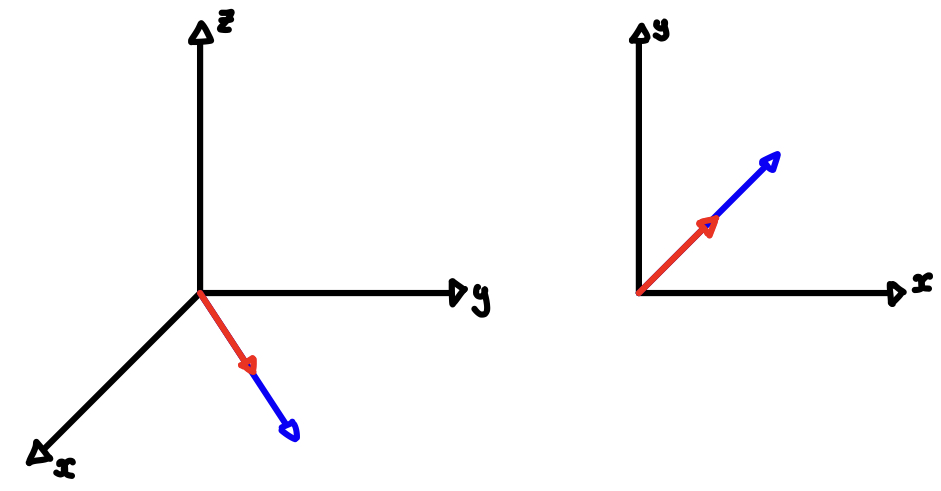
\includegraphics[width=0.90\linewidth]{Modeling-Of-Depolarizing-Channel.jpeg}
\end{center}
\end{figure}
\end{frame}
%------------------------------------------------
%	Quantum Estimation (QFI of Depolarizing Channels)
%------------------------------------------------
\begin{frame}
\frametitle{QFI of Depolarizing Channels}
We now examine the simplest depolarizing channel evolution.
\begin{figure}
\begin{center}
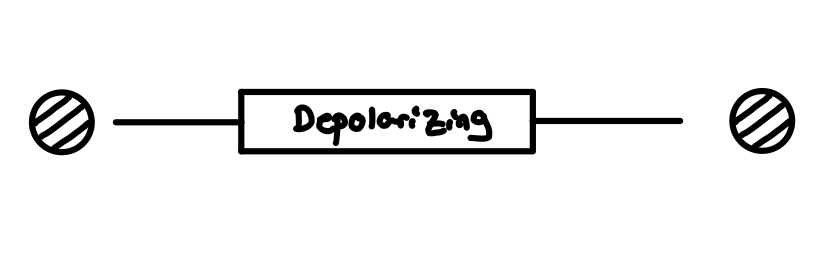
\includegraphics[width=0.75\linewidth]{Depolarizing-Single-Channel-Lambda-Schematic.jpg}
\end{center}
\end{figure}
The Quantum Fisher Information is
\begin{equation}\label{eq:46}
H=\frac{r^2}{1-r^2\lambda^2}.
\end{equation}
\end{frame}
%------------------------------------------------
%	Quantum Estimation (QFI of Depolarizing Channels)
%------------------------------------------------
\begin{frame}
\frametitle{QFI of Depolarizing Channels}
We now examine the next scenario with two particles and one channel depolarizing evolution.
\begin{figure}
\begin{center}
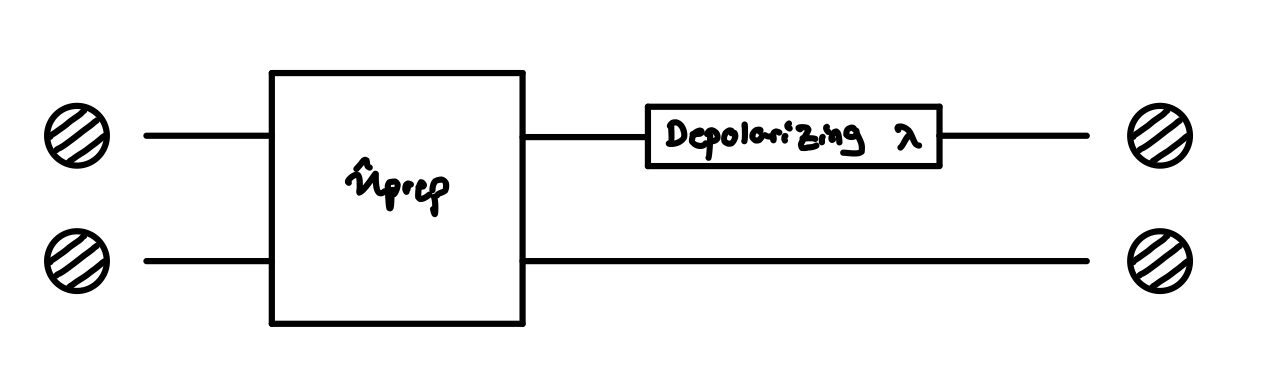
\includegraphics[width=0.75\linewidth]{Depolarizing-Double-Channel-Lambda-Schematic.jpg}
\end{center}
\end{figure}
The Quantum Fisher Information is
\begin{equation}\label{eq:47}
H=\frac{r^2(r^2(1-4\lambda)+r^4\lambda+2)}{(1+2r\lambda+r^2\lambda)(1-2r\lambda+r^2\lambda)(1-r^2\lambda)}.
\end{equation}
\end{frame}
%------------------------------------------------
%	Quantum Estimation (QFI of Depolarizing Channels)
%------------------------------------------------
\begin{frame}
\frametitle{QFI of Depolarizing Channels}
The gain of the last two scenarios is
\begin{equation}\label{eq:48}
G=\frac{(r^2\lambda^2-1)(r^4\lambda-4r^2\lambda+r^2+2)}{(1+2r\lambda+r^2\lambda)(1-2r\lambda+r^2\lambda)(r^2\lambda-1)}.
\end{equation}
\begin{figure}
\begin{center}
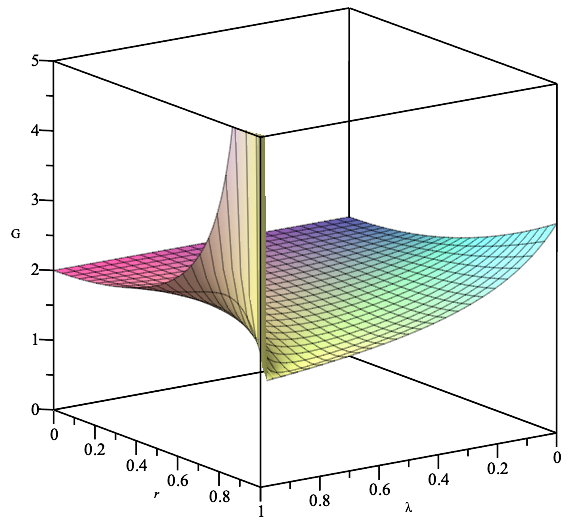
\includegraphics[width=0.60\linewidth]{Depolarizing-Double-Channel-Lambda-Gain-Graph.png}
\end{center}
\end{figure}
\end{frame}
%------------------------------------------------
%	Quantum Estimation (QFI of Depolarizing Channels)
%------------------------------------------------
\begin{frame}
\frametitle{QFI of Depolarizing Channels}
We now examine a two particle two channel depolarizing evolution.
\begin{figure}
\begin{center}
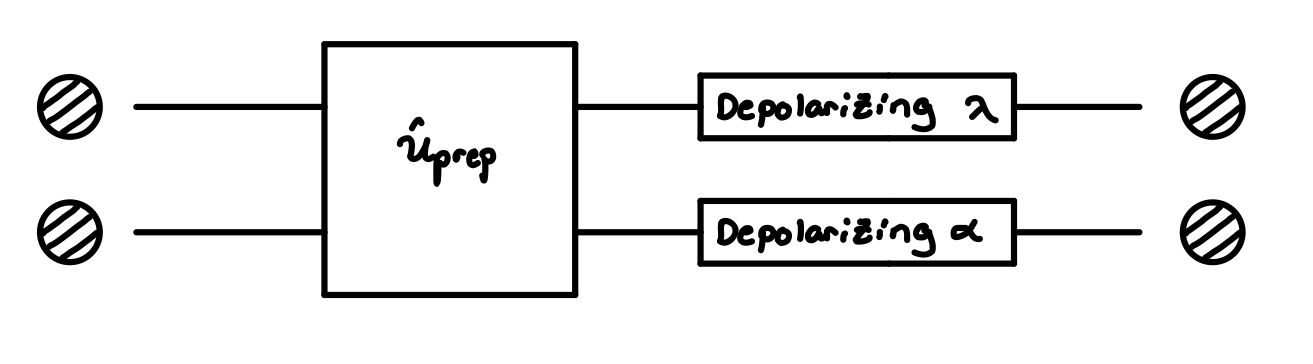
\includegraphics[width=0.75\linewidth]{Depolarizing-Double-Channel-Alpha-and-Lambda-Schematic.jpg}
\end{center}
\end{figure}
The Quantum Fisher Information is
\begin{equation}\label{eq:49}
H=\frac{r^2\alpha^2(\alpha\lambda r^4-4r^2\lambda\alpha+r^2+2)}{(1-r^2\lambda\alpha)(1+r\alpha(r+2)\lambda)(1+r\alpha(r-2)\lambda)}.
\end{equation}
\end{frame}
%------------------------------------------------
%	Quantum Estimation (QFI of Depolarizing Channels)
%------------------------------------------------
\begin{frame}
\frametitle{QFI of Depolarizing Channels}
The gain of the last scenario is
\begin{equation}\label{eq:50}
G=\frac{\alpha(\alpha\lambda r^4-4\lambda r^2\alpha+r^2+2)^2(r^2\lambda^2-1)}{(\lambda r^2\alpha-1)(1+r\alpha(r+2)\lambda)(1+r\alpha(r-2)\lambda)}.
\end{equation}
With $r=0.01$.
\begin{figure}
\begin{center}
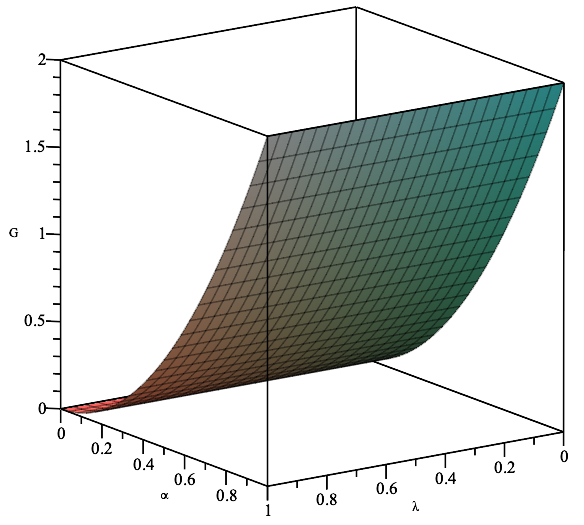
\includegraphics[width=0.60\linewidth]{Depolarizing-Double-Channel-Alpha-and-Lambda-r=001-Gain-Graph.png}
\end{center}
\end{figure}
\end{frame}
%------------------------------------------------
%	Quantum Estimation (QFI of Depolarizing Channels)
%------------------------------------------------
\begin{frame}
\frametitle{QFI of Depolarizing Channels}
With $r=1.0$.
\begin{figure}
\begin{center}
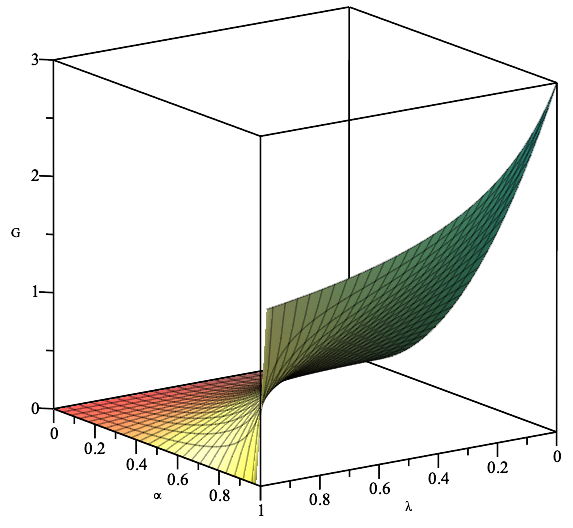
\includegraphics[width=0.75\linewidth]{Depolarizing-Double-Channel-Alpha-and-Lambda-r=1-Gain-Graph.png}
\end{center}
\end{figure}
\end{frame}
%------------------------------------------------
%	Quantum Estimation (QFI of 3 Phase Flip Channels)
%------------------------------------------------
\subsection{\tiny{3 Channel Phase Flip}}
\begin{frame}
\frametitle{QFI of 3 Phase Flip Channels}
We now examine a three particle measurement.
\begin{figure}
\begin{center}
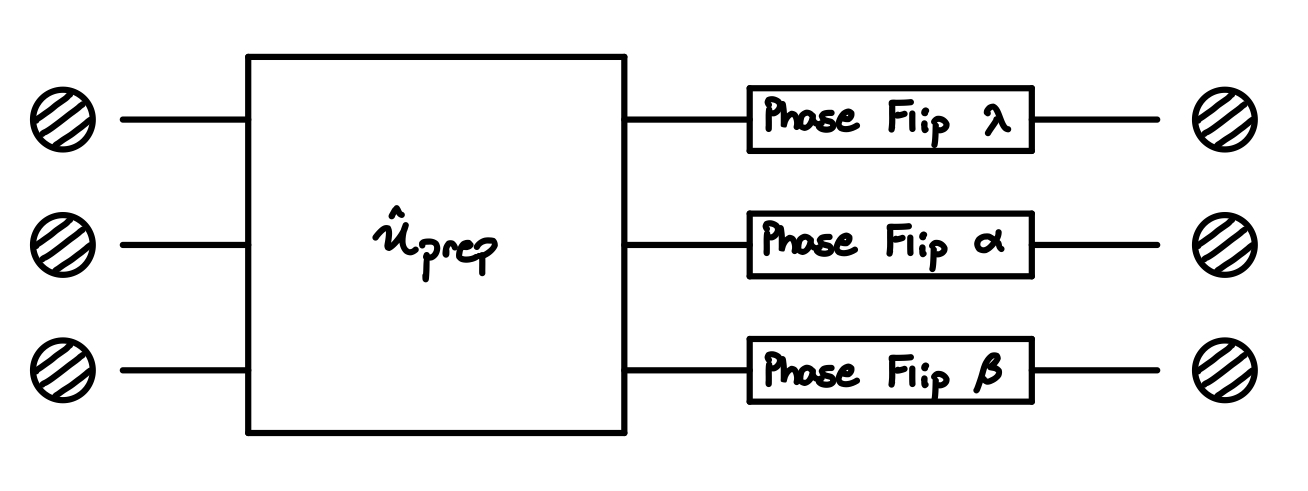
\includegraphics[width=0.75\linewidth]{Phase-Flip-Triple-Channel-Lambda-Schematic.jpg}
\end{center}
\end{figure}
\end{frame}
%------------------------------------------------
%	Quantum Estimation (QFI of 3 Phase Flip Channels)
%------------------------------------------------
\begin{frame}
\frametitle{QFI of 3 Phase Flip Channels}
The Quantum Fisher Information of this measurement comes out to be
\begin{align}\label{eq:45}
H&=r^2(1-2\alpha)^2(1-2\beta)^2\cdot \nonumber \\
\bigg(&\frac{(r+3)^2(3r^2+1)(\eta)+3(1-r^2)^3(\xi)}{(\eta)(\xi)}\bigg)
\end{align}
where $\eta=(1-r^2)^2-\gamma^2r^2(1-r^2)^2$, $\xi=(3r^2+1)^2-r^2(r+3)^2\gamma^2$, and $\gamma=(1-2\lambda)(1-2\alpha)(1-2\beta)$. 
\end{frame}
%------------------------------------------------
%	Quantum Estimation (QFI of 3 Phase Flip Channels)
%------------------------------------------------
\begin{frame}
\frametitle{QFI of 3 Phase Flip Channels}
The gain of the three particle scenario comes out to be
\begin{align}\label{eq:46}
G&=\frac{1-r^2(1-2\lambda)^2(1-2\alpha)^2(1-2\beta)^2}{4}\cdot \nonumber \\
\bigg(&\frac{(r+3)^2(3r^2+1)(\eta)+3(1-r^2)^3(\xi)}{(\eta)(\xi)}\bigg).
\end{align}
With the next gain scenarios $r=0.01$.
\end{frame}
%------------------------------------------------
%	Quantum Estimation (QFI of 3 Phase Flip Channels)
%------------------------------------------------
\begin{frame}
\frametitle{QFI of 3 Phase Flip Channels}
With $\alpha=0.01$.
\begin{figure}
\begin{center}
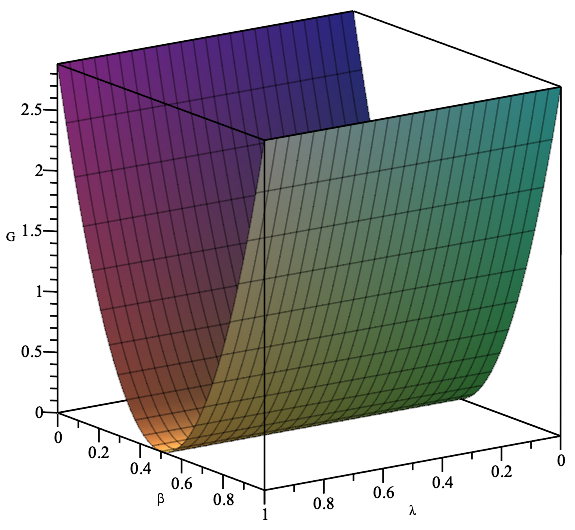
\includegraphics[width=0.75\linewidth]{Phase-Flip-Triple-Channel-r=001-Alpha=001-Gain-Graph.png}
\end{center}
\end{figure}
\end{frame}
%------------------------------------------------
%	Quantum Estimation (QFI of 3 Phase Flip Channels)
%------------------------------------------------
\begin{frame}
\frametitle{QFI of 3 Phase Flip Channels}
With $\beta=0.01$.
\begin{figure}
\begin{center}
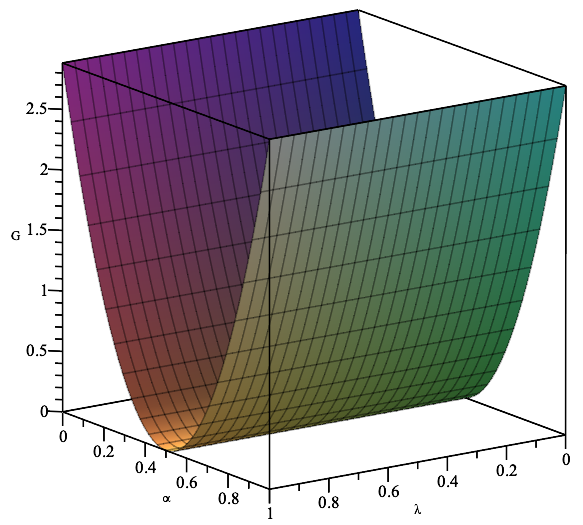
\includegraphics[width=0.75\linewidth]{Phase-Flip-Triple-Channel-r=001-Beta=001-Gain-Graph.png}
\end{center}
\end{figure}
\end{frame}
%------------------------------------------------
%	Quantum Estimation (QFI of 3 Phase Flip Channels)
%------------------------------------------------
\begin{frame}
\frametitle{QFI of 3 Phase Flip Channels}
With this last scenario, $\alpha=0.01$ and $\beta=0.01$.
\begin{figure}
\begin{center}
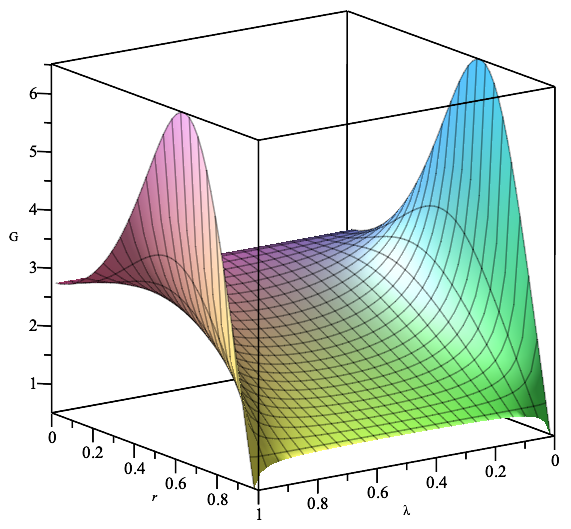
\includegraphics[width=0.75\linewidth]{Phase-Flip-Triple-Channel-Alpha=001-Beta=001-Gain-Graph.png}
\end{center}
\end{figure}
\end{frame}
%----------------------------------------------------------------------------------------------------------------------------------------------------
%------------------------------------------------
%	Conclusion
%------------------------------------------------
\section{Conclusion}
\begin{frame}
\frametitle{Conclusion}
In the presence of Phase Shifts, Phase Flips, and Depolarizing Channels the Quantum Fisher Information will vary depending on initial conditions. \\
\vspace{10pt}
Pure states are difficult to obtain, so in practicality noisy states are commonly used for estimation. \\
\vspace{10pt}
Typically the use of multiple particles in a measurement yield better outcomes with some exceptions.
\end{frame}
%----------------------------------------------------------------------------------------------------------------------------------------------------
%------------------------------------------------
%	References
%------------------------------------------------
\section{References}
\begin{frame}
\frametitle{References}
\footnotesize{
\begin{thebibliography}{99}
\bibitem{Braunstein}
Braunstein, S. L., \& Caves, C. M. (1994). Statistical distance and the geometry of quantum states. Physical Review Letters, 72(22), 3439?3443. doi: 10.1103/physrevlett.72.3439
\bibitem{Caves}
Caves, C. M. (1981). Quantum-mechanical noise in an interferometer. Physical Review D, 23(8), 1693?1708. doi: 10.1103/physrevd.23.1693
\bibitem{D. Collins}
Collins, D. (2019). Qubit-channel metrology with very noisy initial states. Physical Review A, 99(1). doi: 10.1103/physreva.99.012123
\bibitem{Hazewinkel}
Hazewinkel, M. (1995). Encyclopaedia of mathematics. an updated and annotated translation of the soviet "Mathematical encyclopaedia". Dordrecht: Kulver academic.
\bibitem{Helstrom}
Helstrom, C. W. (1969). Quantum detection and estimation theory. Journal of Statistical Physics, 1(2), 231?252. doi: 10.1007/bf01007479
\bibitem{Paris}
Paris, M. G. A. (2009). Quantum state and process estimation. Quantum Information, 139?146. doi: 10.1007/978-0-387-36944-08
\end{thebibliography}
}
\end{frame}
%----------------------------------------------------------------------------------------------------------------------------------------------------
%------------------------------------------------
%	Questions
%------------------------------------------------
\section{Questions}
\begin{frame}
\frametitle{Questions?}
Any Questions?
\end{frame}
\end{document}
%----------------------------------------------------------------------------------------------------------------------------------------------------
%----------------------------------------------------------------------------------------
%	Comment Headers
%----------------------------------------------------------------------------------------

%----------------------------------------------------------------------------------------------------------------------------------------------------

%----------------------------------------------------------------------------------------

%------------------------------------------------

%----------------------------------------------------------------------------------------
%	
%----------------------------------------------------------------------------------------

%------------------------------------------------
%	
%------------------------------------------------
